\chapter{State of the Art}
\label{chap2}
% \thispagestyle{fancy}
\textit{This chapter presents a comprehensive review of the literature, evaluating the current advances in the fields and identifying research gaps in the control of soft quadruped robots with the model-based reinforcement learning.}

\section{Robot Control}
Robot control, especially for soft quadruped robots with a much higher degree of freedom than traditional quadruped robots, is a vital discipline that encompasses the movement and interaction of robots with their surroundings, enabling them to navigate complex terrains effectively\cite{biswalDevelopmentQuadrupedWalking2021}. Typically, the process of implementing control for a robot involves a hierarchical approach\cite{fazeliSeeFeelAct2019}, which initiates with the lower-level control mechanisms and subsequently advances to more complex, task-specific controls. A representation of this hierarchical control structure in quadruped robots is provided in Figure \ref{fig:hierarchy}. However, the hierarchy is not always concrete, different control methods can be employed for different subsystems of the robot.

At the lowest level, control of actuators, primarily motors, is achieved by developing firmware or low-level code\cite{yangMagneticActuationSystems2020}, which enables precise task manipulation and regulates key parameters such as motor speed, rotation direction, or torque. This crucial aspect of motor control can be further integrated into a broader system, directly influencing the robot's kinematics and dynamics\cite{dingNovelDynamicLocomotion2020}. By considering the robot's mechanical structure through the application of kinematics and dynamics principles, control of robot body can be enabled by factoring in joint angles, leg positions, and forces exerted by a rigid quadruped robot\cite{leeLearningQuadrupedalLocomotion2020}. Ideally, this aspect of robot kinematics and dynamics also extends to the orchestration of the robot's gait patterns, enabling more coordinated and efficient locomotion, but some are not\cite{dingNovelDynamicLocomotion2020}. 

Once these lower-level controls are established, the robot can achieve locomotion and perform basic movements. The incorporation of mid-level controls within the robot's control system endows the robot with enhanced capabilities and increased autonomy\cite{choiLearningQuadrupedalLocomotion2023}, wherein most controls in this level aims to optimize the performance. For instance, trajectory control methodologies\cite{leeTrajectoryDesignControl2017}, which are of significant value for tasks necessitating precise positioning or adherence to specific motion profiles, permit the robot to adhere to predetermined routes or execute exact movements with precision and smoothness. Stability control strategies allow the robot to sustain balance and stability\cite{sunBalanceControlQuadruped2022}, even amidst challenging environments or during dynamic motions, thereby mitigating the possibility of instability or the risk of falling. Incorporated obstacle avoidance mechanisms within the robot's control system allow it to perceive environmental obstructions\cite{liQuadrupedRobotObstacle2022}, generate optimal paths or control signals to bypass them, thus ensuring its safe, collision-free navigation and improved efficiency in traversing complex environments. 

Finally, task-specific control strategies can be implemented, designating the comprehensive goals that the robot should accomplish. The strategic level represents the apex of the hierarchical structure of robot control systems and in essence, it centralizes on "what" the tasks are rather than "how" to carry them out. This involves complex high-level planning and decision-making\cite{mikiLearningRobustPerceptive2022}, which are later converted into specific actions at lower levels. The comprehensive understanding and systematic implementation of these control mechanisms enable the development of robotic systems capable of precise and Optimal control in diverse environments and applications. 
\usetikzlibrary{shapes,arrows,positioning,calc}
\begin{figure}[ht]
\centering
    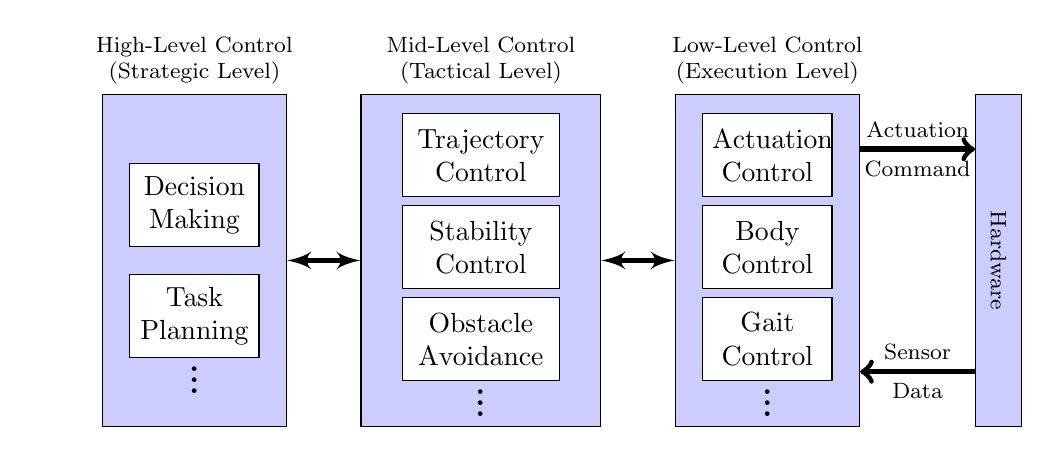
\begin{tikzpicture}[
        node distance = 3cm,
        auto,
        block/.style = {rectangle, draw, fill=blue!20, text width=8em, minimum height=12em},
        block0/.style = {rectangle, draw, fill=blue!20, text width=6em, minimum height=12em},
        block1/.style = {rectangle, draw, fill=blue!20, text width=1em, minimum height=12em},
        smallblock/.style = {rectangle, draw, fill=white, text width=5em, text centered, minimum height=3em},
        smallblock0/.style = {rectangle, draw, fill=white, text width=4em, text centered, minimum height=3em},
        line/.style = {draw, -latex'}
    ]
    
        % Place nodes
        \node [block0] at (0,0)(high) {};
        \node[align=center, font=\footnotesize, above=0em of high, text width=4cm]{High-Level Control\\ (Strategic Level)};
        \node [smallblock0] at ($(high.center) + (0, 2em)$) (highsub1) {Decision Making};
        \node [smallblock0] at ($(high.center) + (0,-2em)$) (highsub2) {Task Planning};
        \node [font=\huge] at ($(highsub2.south) + (0,-0.5em)$) {\vdots};
        
        \node [block] at ($(high.east) + (7em,0)$) (mid) {};
        \node[align=center, font=\footnotesize, above=0em of mid, text width=4cm]{Mid-Level Control \\ (Tactical Level)};
        \node [smallblock] at ($(mid.center) + (0,3.8em)$) (midsub1) {Trajectory Control};
        \node [smallblock] at ($(midsub1.south) + (0,-1.8em)$) (midsub2) {Stability Control};
        \node [smallblock] at ($(midsub2.south) + (0,-1.8em)$) (midsub3) {Obstacle Avoidance};
        \node [font=\huge] at ($(midsub3.south) + (0,-0.5em)$) {\vdots};

        \node [block0] at ($(mid.east) + (6em,0)$)(low) {};
        \node[align=center, font=\footnotesize, above=0em of low, text width=4cm]{Low-Level Control\\ (Execution Level)};
        \node [smallblock0] at ($(low.center) + (0,3.8em)$) (lowsub1) {Actuation Control};
        \node [smallblock0] at ($(lowsub1.south) + (0,-1.8em)$) (lowsub2) {Body Control};
        \node [smallblock0] at ($(lowsub2.south) + (0,-1.8em)$) (lowsub3) {Gait Control};
        \node [font=\huge] at ($(lowsub3.south) + (0,-0.5em)$) {\vdots};
        
        \node [block1] at ($(low.east) + (5em,0)$) (hardware) {};
        \node[rotate=-90, align=center, font=\footnotesize]at (hardware.center){Hardware};
        
        % % Draw edges
        \draw [line width=2pt, >=latex', <->] (high.east) -- (mid.west);
        \draw [line width=2pt, >=latex', <->] (mid.east) -- (low.west);
        \draw [line width=2pt,->] ($(low.north east) + (0,-2em)$) -- node[font=\footnotesize,above] {Actuation}node[font=\footnotesize,below] {Command}($(hardware.north west) + (0,-2em)$);
        \draw [line width=2pt,->] ($(hardware.south west) + (0,2em)$) -- node[font=\footnotesize,above] {Sensor}node[font=\footnotesize,below] {Data}($(low.south east) + (0,2em)$);
    
    \end{tikzpicture}
    \caption{Hierarchical control levels in quadruped robots.}
    \label{fig:hierarchy}
\end{figure}


The control of soft quadruped robots is an area of active research due to the inherent difficulties involved. The KTH soft quadruped robot SoftQ represents a significant advancement in this field, and this thesis aims to contribute to its control system development at the lower-level control hierarchy, specifically motion control, gait control, and body control, there are several key considerations and techniques that can be explored to enable walking and achieve stable locomotion. 

\subsection{Kinematics and Dynamics}
Kinematics and dynamics are two fundamental aspects of robotic systems that are closely related to motion control. Kinematics refers to the study of the geometric properties of motion without considering the forces or torques involved. In the case of rigid quadruped robots, kinematics focuses on determining the relationships between joint angles, leg positions, and the resulting end-effector positions and orientations. In the context of soft robots, kinematics involves understanding the relationships between deformations in the robot's soft structure and the resulting end-effector positions and orientations. By comprehending the kinematics of soft robots, it becomes possible to calculate the deformations required to achieve specific end-effector poses. The kinematic equations for soft robots can be challenging to derive due to the complex and deformable nature of their structures. Traditional kinematic models used for rigid robots, such as transformation matrices and \ac{D-H} parameters, may not be directly applicable to soft robots\cite{fangKinematicsSoftRobots2020}. Instead, with precise modeling formulation of soft materials, \ac{FEA}\cite{leeFEMbasedSoftRobotic2017} and the Jacobian method of statics\cite{giorelliNeuralNetworkJacobian2015} have been employed to accurately model the kinematics of soft robots. However, it is worth noting that these advanced methods can be computationally expensive, particularly when used in conjunction with \ac{RL} training processes. 

Dynamics, on the other hand, involves the study of the forces and torques that influence the robot's motion. In the context of quadruped robots, dynamics principles help in understanding how the forces and torques at each joint and leg affect the overall motion and stability of the robot. By modeling the dynamics of the system, one can accurately predict the forces and torques required to achieve desired motions or maintain balance. One of the famous models used to describe the locomotion dynamics of legged robots is the \ac{SLIP} model\cite{poulakakisSpringLoadedInverted2009}, which approximates a legged system as a single mass with a spring and/or a damper and it exhibits simplicity and effectiveness in capturing the fundamental dynamics of hopping and running.

Furthermore, control in robotics involves various models, from simple templates to a full rigid body model, a wide range of models existed to control quadruped robot in practice\cite{hwangboSimulationRealWorld2018}. However, when it comes to soft quadruped robots, modeling them with simple kinematics and dynamics functions becomes challenging due to the presence of hysteresis,nonlinearity and other complex factors. Despite some research teams from KTH\cite{daneliaStructureGaitOptimizationof2021, lagreliusComparingFourModelling2022} have successfully incorporated factors such as flexible body dynamics, non-linear material properties, and complex joint constraints, a research gap still exists in the development of real-time solutions, as existing models can be computationally expensive, limiting their practical applications.

\subsection{Gait Control}
By analyzing the kinematics and dynamics of robots, it is possible for us to identify gait patterns, joint coordination strategies, or control parameters that enhance the locomotion performance. In the case of quadruped robots, gait control plays a crucial role in coordinating leg movements for effective locomotion, which can be roughly categorized into two groups:  modular design by employing the heuristic and optimal design to minimize the cost. 

A modular controller approach involves breaking down a complex control problem into smaller, more manageable subproblems. Each subproblem is then addressed by a specific control module, which has a well-defined input-output interface and can be replaced or modified to generate different behaviors. Many research teams have developed modular controllers for specific robots\cite{hutterANYmalHighlyMobile2016,bledtMITCheetahDesign2018,jiOmnidirectionalWalkingQuadruped2022}, achieving impressive performance in locomotion and dynamic gaits. Despite their success, modular controller designs have certain limitations. Firstly, the development process is time-consuming and complex, requiring significant expertise and modifications for different tasks. Secondly, the simplifications and lack of accounting for coupling effects between modules can lower overall control performance, especially in dynamic maneuvers. Lastly, optimizing the contact schedule, a plan for when the robot's parts touch the ground, remains a challenging problem that current algorithms cannot handle\cite{bledtContactModelFusion2018}. As a result, most controllers resort to heuristic or hand-coded contact schedules.

The optimization-based gait control utilizes an effective cost function within a single optimization framework to find optimal motions for diverse tasks without a specific architecture for each task. The optimization of smooth and convex objective functions with multiple linear constraints has been extensively studied and is well-established in various fields of applied mathematics\cite{koldaOptimizationDirectSearch2003}. However, when it comes to planning trajectories for legged systems, the complexity of the problem poses significant challenges, and common optimization approaches are often not directly applicable. One key challenge in trajectory planning for legged systems is the need to consider multiple possible contact points with the environment. To simplify the problem, many existing algorithms make strong assumptions, such as limiting the number of contact points\cite{daiWholebodyMotionPlanning2014} and pre-specifying their locations\cite{gehringPracticeMakesPerfect2016}. By reducing the problem to a set of specific contact points, the complexity associated with collision primitives of the robot can be mitigated. Consequently, the task of finding an optimal contact trajectory becomes a convex problem that involves considering various combinations. To solve the combinational problems, one popular approach is to "softly" comply with contact dynamics by using a novel cost function\cite{farshidianRealtimeMotionPlanning2017}. Another approach involves predefining the contact sequence and effectively converting the model to a switched system with time-dependent switching\cite{kochOptimizationbasedWalkingGeneration2012}. All these approaches have some sort of limitations, a common criticism of the first approach is that the generated motion may violate physical constraints, leading to a lack of realism and the computational cost for the second approach can be substantial, making online optimization impractical for legged systems. 

As for soft quadruped robots, the challenges and considerations in gait control are further amplified. In the context of soft quadruped robots, gait control methods need to account for the deformations and interactions between the robot's body and the environment. Traditional approaches based on rigid-body dynamics and contact modeling may not be directly applicable in this case. However, the combination of modular design and optimization-based approaches can also be beneficial in gait control for soft quadruped robots. 

\subsection{Whole Body Control}
Whole body control is a comprehensive approach that considers the robot as a whole system, coordinating the movements of all its limbs and body to achieve desired behaviors and tasks while accounting for interactions with the environment. By combining modular design and optimization-based approaches, whole body control capitalizes on the strengths of both methods. Modular design offers modularity and reusability of control modules, facilitating efficient development and behavior modification. On the other hand, the optimization-based approach provides flexibility and adaptability to various tasks and environments, enabling the generation of optimal control signals.These control architectures have demonstrated impressive performance on real systems. For instance, some research groups\cite{kalakrishnanFastRobustQuadruped2010,bledtMITCheetahDesign2018} have successfully implemented such a controller for the quadruped robot, LittleDog and Mini Cheetah(Fig.\ref{fig:LittleDog}). Their controller comprised five modules: a footstep planner, a pose finder, a body trajectory generator, a foot trajectory planner, and a tracking controller. Each module produces desired values of physical quantities. This controller achieved significant success in the challenge program\cite{neuhausComprehensiveSummaryInstitute2011}, Learning Locomotion (L2) from Defense Advanced Research Projects Agency (DARPA) and remains a state-of-the-art approach in rough-terrain legged locomotion control even after a decade of research.
\begin{figure}[htb]
\centering
    \begin{subfigure}[b]{0.45\textwidth}
    \centering 
        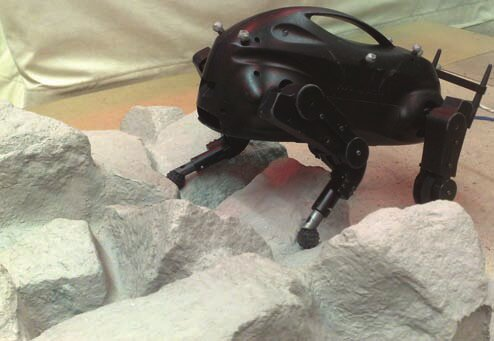
\includegraphics[height=0.6\linewidth]{img/chap2/LittleDog.jpg}
        \caption{}
    \end{subfigure}
    \begin{subfigure}[b]{0.45\textwidth}
    \centering
        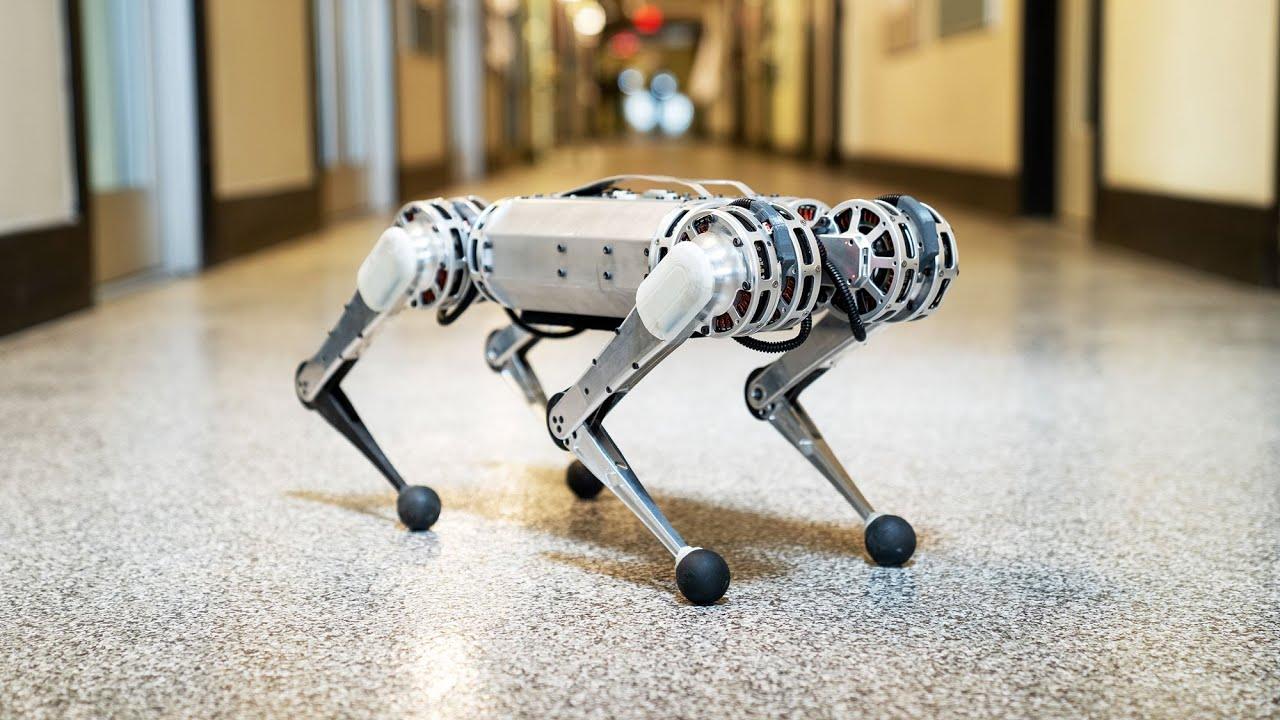
\includegraphics[height=0.6\linewidth]{img/chap2/minicheetah.jpg}
        \caption{}
    \end{subfigure}
    \caption{Rigid quadruped robot named (a) LittleDog\cite{kalakrishnanFastRobustQuadruped2010} and (b) Mini Cheetah\cite{bledtMITCheetahDesign2018}, both have whole body controllers implemented.}
    \label{fig:LittleDog}
\end{figure}


In soft quadruped robots, gait control becomes even more challenging due to the complex and compliant nature of the robot's body, which also applies to the broader concept of whole body control. Soft robots require novel approaches to gait control that consider factors such as the interaction between soft materials, real-time sensing, and adaptation to varying terrain and environmental conditions. The integration of advanced control mechanisms, as discussed above, serves as a solid foundation for the introduction of robot learning into the control framework. By integrating these factors into the control system and leveraging machine learning techniques, it is possible to achieve stable and efficient locomotion in soft robots. Ongoing research in this area aims to develop advanced gait control strategies for soft quadruped robots, pushing the boundaries of their locomotion capabilities\cite{gongReviewGaitOptimization2010}.

\section{Robot Learning}
While control algorithms govern robot behavior, robot learning complements this by enabling robots to acquire knowledge and improve their control strategies through experience and interaction with the environment. By incorporating supervised learning techniques, robots can go beyond pre-programmed behaviors and adapt their control policies based on real-time sensory information and learned models\cite{whiteheadLearningPerceiveAct1991}. Robot learning refers to the ability of a robot to acquire knowledge and improve its performance through experience, interaction with the environment, and data-driven methods. It involves enabling robots to learn from their own actions, from human guidance, or from analyzing large amounts of data. The goal of robot learning is to equip robots with the ability to adapt, generalize, and improve their behavior over time without being explicitly programmed for every possible scenario. Robot learning empowers robots to autonomously acquire new skills, optimize their performance, and adapt to novel situations, enhancing their adaptability, flexibility, and efficiency. 

By combining the principles of robust control with the capabilities of robot learning, the field of robotics continues to advance, striving to develop intelligent and optimal systems that can autonomously learn, adapt, and perform complex tasks in dynamic and uncertain environments. It is worth noting that the field of gait control for quadruped robots is continuously evolving, and researchers are actively exploring new approaches to control the gait of different robots. Among these approaches\cite{nakamuraReinforcementLearningBiped2007, wangHierarchicalGaitGeneration2021, leeQuadrupedRobotObstacle2006, choiLearningQuadrupedalLocomotion2023}, some utilize a parameterized control policy representation, where the parameters can be optimized using learning-based methods or hand-tuned. Two particularly popular approaches in this direction are \ac{CPG} and \ac{RL}. The categorization here was based on historical perspectives rather than fundamental differences.

\subsection{Central Pattern Generator}
\begin{figure}[htb]
    \centering
    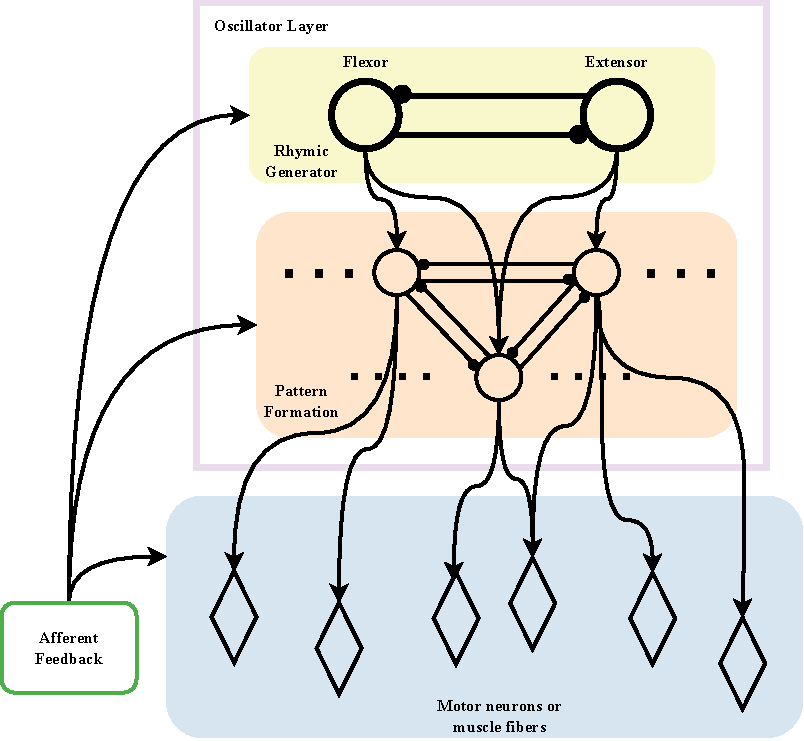
\includegraphics[width=0.7\linewidth]{img/chap2/CPG.pdf}
    \caption{Schematic illustration of hypothetical \ac{CPG} structure for mammalian movement control, reproduced from Li et al.\cite{liHumanoidsLearningWalk2013}}
    \label{fig:cpg_structure}
\end{figure}

\ac{CPG} in robot can be thought of as a scheduler, responsible for a rhythmic pattern of leg movements that enables the robot to move in a coordinated manner. Originally found in the spinal cords of animals, \ac{CPG}s provide the fundamental neural control required to generate rhythmic muscle activations, which drive various forms of locomotion like walking, running, or swimming. The Figure \ref{fig:cpg_structure} depicts a three-level \ac{CPG} concept from human for locomotion. It consists of a half-center rhythm generator, a pattern formation network, and a motor neuron layer. The yellow area represents the rhythmic generator layer with oscillators producing rhythmic signals as input to the pattern formation layer. The red area represents the pattern formation network, which contains interneuron populations that distribute and synchronize the rhythmic input to motor neuron pools via inhibitory connections. The motor neuron layer integrates sensory feedback and pattern formation network outputs to determine muscle activation. These networks demonstrate a fundamental understanding of how neural networks can generate rhythmic patterns for coordinated leg movements during locomotion. By emulating the functionality of \ac{CPG}s, a gait control mechanisms for quadruped robots were successfully developed in a pioneering works\cite{sprowitzDynamicTrotGait2013}, and it also plays an important role in recent advanced quadruped robots like the MIT Cheetah\cite{dicarloDynamicLocomotionMIT2018}. \ac{CPG}s can be regarded as a specialized neural networks to generate the rhythmic patterns that facilitate locomotion. \ac{ANN}s are computational models that emulate the architecture and functionality of biological neural networks, comprising interconnected nodes (neurons) that process and transmit information using weighted connections. Given the shared structural characteristics between \ac{CPG}s and \ac{ANN}s, it is common to consider the application of the training methods developed for \ac{ANN}s to some \ac{CPG}s. 


\subsection{Reinforcement Learning}
Unlike other approaches, \ac{RL} is built upon a flexible problem framework that can effectively handle various control challenges,  includes a diverse range of scenarios such as stochastic, nonlinear, nonconvex, and nonsmooth problems, if sufficient training samples are available. Moreover, one of the key strengths of \ac{RL} is its ability to tackle complex control tasks without relying on control architectures manually crafted by humans. Instead, \ac{RL} only need a general approximation (e.g., a deep neural network) to learn and optimize control policies autonomously, degrading the need for extensive human design efforts. \ac{RL} is a subfield of machine learning that focuses on how an agent can learn to make optimal decisions through interaction with an environment. It is inspired by the way humans and animals learn from trial and error to achieve desired goals. While employing \ac{RL} approaches, the agent is designed to execute actions that maximize cumulative rewards within a defined time horizon. By assigning rewards or penalties based on the robot's performance, the algorithms will iteratively adjust the control policies to optimize the desired behavior. Through repeated interactions with the environment, the robot can learn to generate effective gaits and adapt to different terrains and disturbances. This approach has shown promising results in achieving dynamic and robust locomotion for quadruped robots\cite{jiConcurrentTrainingControl2022}. 

As the complexity of robotics increases, \ac{RL} is increasingly required to develop robust control algorithms with high \ac{DoF}s and time variant properties\cite{zhangEffectiveSoftRobot2017}. The rapid development of AI provides an alternative solution to take into account the nonlinear properties of novel materials and soft robots\cite{tangModelbasedOnlineLearning2021}. In the reinforcement learning era, many new algorithms tailored for continuous control of robot have made it possible to learn to perform complex tasks. These algorithms, such as \ac{SAC}\cite{haarnojaSoftActorCriticOffPolicy2018} and Deep Deterministic Policy Gradient (DDPG)\cite{silverDeterministicPolicyGradient2014}, have been successful in enabling continuous control in reinforcement learning\cite{haarnojaLearningWalkDeep2019, pengSimtoRealTransferRobotic2018}. DDPG is a popular algorithm for continuous control. DDPG combines the power of deep neural networks with the deterministic policy gradient algorithm. Through the training process, DDPG learns an actor network, responsible for directly mapping states to actions, and a critic network, which estimates the expected return\cite{silverDeterministicPolicyGradient2014}. SAC is an off-policy algorithm that utilizes maximum entropy reinforcement learning to encourage exploration\cite{haarnojaSoftActorCriticOffPolicy2018}. This algorithm excels in scenarios with continuous action spaces\cite{haarnojaLearningWalkDeep2019}, making it highly suitable for a wide range of robotic control tasks. By optimizing a stochastic policy and simultaneously learning a value function to estimate the expected return, SAC achieves effective exploration and robust learning\cite{haarnojaLearningWalkDeep2019, pengSimtoRealTransferRobotic2018}. Therefore, Ji et al. \cite{jiSynthesizingOptimalGait2022} selected \ac{SAC} to train the robot to walk for better exploration efficiency and suitability for continuous action spaces.

\subsubsection{Model-based Reinforcement Learning}
Although Ji et al.\cite{jiSynthesizingOptimalGait2022}'s controller showed promising results, achieving an effective policy may still require prolonged training over several days or even weeks. The algorithm they proposed belongs to the category of \ac{MFRL}, which involves complex simulations and can be significantly slowed down by them. In \ac{MBRL}, an agent learns optimal behavior by creating a model of the environment through action and observation. Instead of explicitly modeling the environment, MBRL agents make decisions based on their experiences and rewards. This approach involves mapping observations to actions without delving into the underlying dynamics of the environment. To achieve that, a model of the environment comprising state transition distribution ($P_\eta$) and reward function ($R_\eta$) is created in MBRL.
\begin{figure}[ht]
\centering
    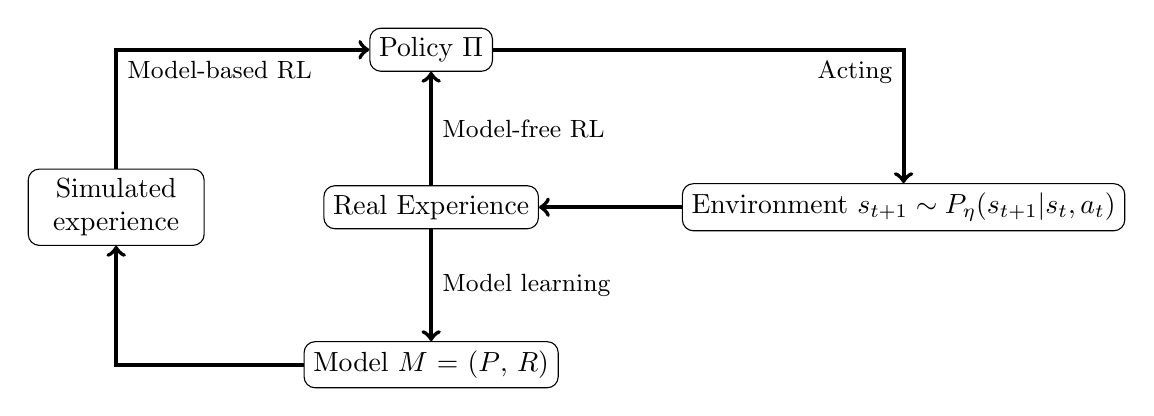
\begin{tikzpicture}[node distance=2cm, auto]
        % Define nodes
        \node (policy) [rounded corners, draw] {Policy $\Pi$};
        \node (real_experience) [rounded corners, draw, below of=policy] {Real Experience};
        \node (environment) [rounded corners, draw, right of=real_experience, node distance=6cm] {Environment $s_{t+1}\sim P_\eta(s_{t+1}|s_t, a_t)$};
        \node (model) [rounded corners, draw, below of=real_experience] {Model \ensuremath{M} = (\ensuremath{P}, \ensuremath{R})};
        \node (simulated_experience) [align=center, text width=2cm, rounded corners, draw, left of=real_experience, node distance=4cm] {Simulated experience};
        
        % Draw arrows
        \draw[->, line width=1.5pt] (policy) -| (environment) node[midway, below left, font=\small] {Acting};
        \draw[->, line width=1.5pt] (environment) -- (real_experience);
        \draw[->, line width=1.5pt] (real_experience) -- (model) node[midway, right, font=\small] {Model learning};
        \draw[->, line width=1.5pt] (model) -| (simulated_experience);
        \draw[->, line width=1.5pt] (real_experience) -- (policy) node[midway, right, font=\small] {Model-free RL};
        \draw[->, line width=1.5pt] (simulated_experience) |- (policy) node[font=\small, midway, below right] {Model-based RL};
    \end{tikzpicture}
    \caption{Model-free \ac{RL} vs. Model-based \ac{RL}}
    \label{fig:demo}
\end{figure}


Typically, the model can be considered as a combination of state transition distribution $P_\eta$ and reward function $R_\eta$, $$M = (P,R) \textrm{ where } s_{t+1}\sim P_\eta(s_{t+1}|s_t, a_t) \textrm{ and } r_{t+1}\sim R_\eta(r_{t+1}|s_t, a_t)$$ $s_t$ is the state at time $t$, $r_t$ is the reward at time $t$ and $a_t$ is the action at time $t$.These components capture how the state transitions and rewards evolve as the agent takes actions in the environment. In other words, they describe the agent's interactions with the environment. By utilizing a learned model of the environment, \ac{MBRL} allows for efficient exploration and faster learning. Safety considerations are also addressed, as MBRL allows for risk assessment and the avoidance of potentially harmful actions. In environments with sparse rewards, MBRL shines by generating informative trajectories, mitigating the challenge of exploration.

While MBRL requires the agent to build an abstract model of the environment, it needs to accurately represent the true behavior of the system for effective learning. However, in cases like the simulation of SoftQ conducted in Simulink, It is challenging to train the surrogate model simultaneously with RL training. Thus, the training of a surrogate for a soft quadruped robot interacts with the environment using a data-driven approach.

The training of a gait controller for a soft quadruped robot using a data-driven approach in \ac{MBRL} involves gathering empirical data to inform the control policy. However, an alternative MBRL approach utilizes a model, such as Neural Networks, of the robot and its environment to generate training data swiftly and cost-effectively.  This approach facilitates the exploration of diverse control policies and behaviors while offering scalability and efficiency advantages over a purely data-driven approach. By employing deep learning techniques like neural networks, robots can effectively process and interpret complex sensory data, enabling them to understand and respond to their surroundings more comprehensively.

\subsection{Neural Network}
As a basic type of Neural Networks, \ac{ANN}s are computational models that draw inspiration from the structural and functional characteristics of biological neurons\cite{zhangIntroductionArtificialNeural2000}. The biological neuron serves as the fundamental building block of the nervous system, specifically designed to transmit electrical signals and facilitate signal processing. Its remarkable computational capabilities are evident through its capacity to process and integrate intricate information using electrochemical signaling\cite{zouOverviewArtificialNeural2009}. It excels in generalization and adaptation by extracting shared characteristics from patterns, enabling the application of knowledge to novel scenarios. Additionally, biological neurons exhibit robustness and fault tolerance\cite{chenElectrochemicalMemristorBasedArtificialNeurons}, ensuring reliable information processing even in the presence of noise, damage, or missing data. The parallel processing nature of neural networks enables efficient computation\cite{hopfieldNeuralNetworksPhysical1982}, as multiple neurons can concurrently process information, resulting in swift and simultaneous operations. Hence, emulating the neuron and constructing a network seems highly promising. 

An artificial neuron, as a simplified mathematical model, designed to takes input signals, performs a weighted sum of those inputs, applies an activation function to produce an output, and passes it on to the next layer of neurons, the details is shown as Figure \ref{fig:ann}. The connections between neurons in an ANN are represented by weights, which determine the strength or importance of the signal transmitted between them. This learning process often involves techniques like supervised learning\cite{ebertRobustnessRetryingClosedLoop2018}, unsupervised learning\cite{koenigUnsupervisedLearningProbabilistic1996}, or reinforcement learning\cite{jiSynthesizingOptimalGait2022}. 
\begin{figure}[htb]
    \centering
    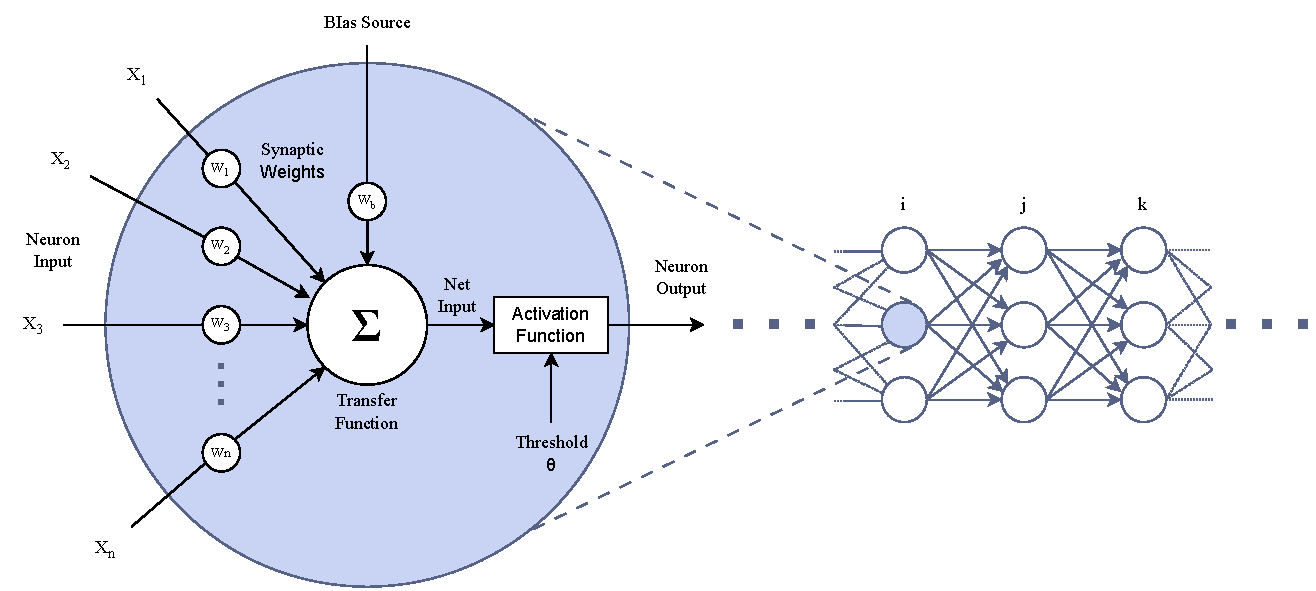
\includegraphics[width=0.9\linewidth]{img/chap2/Neuron.pdf}
    \caption{\ac{ANN} Neuron structure and hidden layers distribution, reproduced from Shashwat et al.\cite{gangulyOptimisedBuildingEnergy2020}}
    \label{fig:ann}
\end{figure}


Furthermore, the development of some advanced architectures and learning algorithms have been developed to address specific challenges. For instance, typical \ac{DNN}, often referred to feed forward neural network, employ a unidirectional flow of data, moving from the input layer to the output layer without revisiting any nodes. This architecture is ideal for tasks that require feature extraction and pattern recognition in static dataset\cite{hwangboLearningAgileDynamic2019}. \ac{CNN} utilizes convolutional layers and pooling layers to automatically capture spatial features and ensure computationally efficient\cite{albawiUnderstandingConvolutionalNeural2017}. \ac{RNN} maintains an internal memory to be able to accommodate variable input lengths benefit them in processing sequential data\cite{liptonCriticalReviewRecurrent2015}. Generative Adversarial Network (GAN) learn to capture underlying patterns and variations in the training data through adversarial training process\cite{songEnergyConsumptionAuditing2023}.   

\section{Inspiration}
In terms of current trends, efficient locomotion and interaction in quadruped robots, including soft quadruped robots with higher degrees of freedom, depend on effective robot control. A commonly employed approach to robot control is the hierarchical framework, or called modular framework, which begins with low-level control of actuators and progresses to higher-level task-specific controls. In specific, the precise control of kinematics and dynamics is crucial for ensuring the robot's movement and stability, while gait control coordinates leg movements to achieve efficient locomotion. Furthermore, the integration of modular frameworks and optimization-based approaches, for the whole body control, enhances the robot's capabilities and autonomy by considering the robot as a cohesive system. Additional control algorithms, robot learning methods such as Central Pattern Generators (CPG) and Reinforcement Learning (RL) enable robots to acquire knowledge and improve their control strategies through experience and interaction with the environment. The utilization of neural networks, such as Artificial Neural Networks (ANN), is prevalent in robot control and learning, enabling robots to effectively model complex relationships between sensory inputs and control outputs, thereby facilitating stable and adaptive gaits.

However, despite the progress made in these areas, certain research gaps still exist. One such gap lies in the realm of real-time solutions for modeling the intricate kinematics and dynamics of soft quadruped robots, as existing models tend to be computationally demanding. Moreover, optimizing gait control for soft quadruped robots, taking into account the intricate interaction between their bodies and the environment, remains a challenging endeavor. Furthermore, while reinforcement learning algorithms exhibit promise in the realm of gait control, achieving an effective policy may necessitate extended training duration. Addressing this challenge could be accomplished through the adoption of model-based reinforcement learning approaches.

In summary, the synthesis of the key findings underscores the vital role that robot control plays in facilitating efficient locomotion and interaction in both rigid quadruped robots but the classic methods might not be able to merged in soft robotics control directly. The existing literature suggests that model-based RL has the potential to develop optimal policies for quadruped robots, including soft quadruped robots. However, the effectiveness of the approach depends on the accuracy of the learned model and the complexity of the environment. In addition, most existing studies have focused on simulated environments, and there is a need for further research on applying model-based RL to physical soft quadruped robots in real-world settings. However, research gaps persist, including the need for real-time solutions for modeling soft quadruped robots and optimizing gait control for their compliant nature. These trends indicate the ongoing exploration of control and learning techniques tailored to soft quadruped robots, with the ultimate goal of enhancing their adaptability and efficiency.